\section{Results}

\subsection{Quantitative Comparison}
\begin{table}[t]
\centering
\small
\caption{Original versus integrated Part 1. Image AUROC is directly
comparable; localization also changes from a 32-pixel patch grid to a common
448 grid.}
\label{tab:integration}
\begin{tabular}{lcccc}
\toprule
Shot & Old image & New image & Old loc. & New loc. \\
\midrule
1 & 51.46 & \textbf{56.37} & 42.99 & \textbf{56.89} \\
2 & 52.79 & \textbf{57.59} & 42.51 & \textbf{57.08} \\
4 & 54.52 & \textbf{58.22} & 41.63 & \textbf{57.82} \\
8 & 56.27 & \textbf{60.71} & 41.58 & \textbf{57.89} \\
\bottomrule
\end{tabular}
\end{table}


Table~\ref{tab:integration} isolates the engineering integration. Multi-channel
differences raise image AUROC by 3.7-4.9 points at every shot count. The
localization increase is larger, but part of it comes from replacing the old
32-pixel patch-grid evaluation with a 448-pixel common grid, so the method and
measurement contributions are not conflated.

At the mandated calibration threshold, the integration lowers test false
positive rate from 32.9-35.1\% to 7.9-10.6\%, but raises false negative rate
from 64.8-70.1\% to 80.3-85.1\%. The integrated baseline is therefore more
conservative: it sharply reduces normal-sample false alarms while missing more
defects. This trade-off is preferable for costly false alarms but is not a
universally better operating point.

\begin{table*}[t]
\centering
\small
\caption{Unweighted category mean and standard deviation over seeds.
Image AUROC is shown in the upper block and patch-level pixel AUROC
in the lower block.}
\label{tab:main}
\begin{tabular}{lcccc}
\toprule
Method & 1-shot & 2-shot & 4-shot & 8-shot \\
\midrule
\multicolumn{5}{l}{\emph{Image-level AUROC (\%)}}\\
Template & 51.5 $\pm$ 1.0 & 52.8 $\pm$ 2.8 & 54.5 $\pm$ 3.7 & 56.3 $\pm$ 1.6 \\
AnomalyDINO & 94.6 $\pm$ 1.0 & 95.3 $\pm$ 0.6 & 96.2 $\pm$ 0.5 & 96.6 $\pm$ 0.7 \\
Multi-layer & 95.0 $\pm$ 0.7 & 95.7 $\pm$ 0.5 & 96.6 $\pm$ 0.6 & 97.0 $\pm$ 0.7 \\
\midrule
\multicolumn{5}{l}{\emph{Patch-level pixel AUROC (\%)}}\\
Template & 43.0 $\pm$ 2.3 & 42.5 $\pm$ 3.8 & 41.6 $\pm$ 3.4 & 41.6 $\pm$ 1.3 \\
AnomalyDINO & 96.4 $\pm$ 0.1 & 96.6 $\pm$ 0.1 & 96.9 $\pm$ 0.0 & 97.0 $\pm$ 0.1 \\
Multi-layer & 96.4 $\pm$ 0.1 & 96.6 $\pm$ 0.0 & 96.9 $\pm$ 0.0 & 97.1 $\pm$ 0.1 \\
\bottomrule
\end{tabular}
\end{table*}


\begin{table*}[t]
\centering
\small
\caption{Per-category image AUROC (\%) at 4-shot, mean over three seeds.}
\label{tab:category}
\begin{tabular}{lcccccc}
\toprule
Method & candle & capsules & cashew & chewinggum & fryum & pipe\_fryum \\
\midrule
Template & 59.3 & 53.7 & 58.6 & 57.0 & 17.4 & 81.1 \\
AnomalyDINO & 92.8 & 98.1 & 93.3 & 99.0 & 97.4 & 96.4 \\
Multi-layer & 93.2 & 98.5 & 94.0 & 99.0 & 97.7 & 96.9 \\
\bottomrule
\end{tabular}
\end{table*}


Figure~\ref{fig:curves} shows the shot scaling. We report mean and standard
deviation over seeds. The integrated template baseline improves substantially
over the original RGB-only version, but it remains sensitive to pose,
illumination, and background variation. AnomalyDINO benefits more consistently
from additional normal views because rotation augmentation and patch-level
matching approximate the local normal manifold.

\begin{figure}[t]
\centering
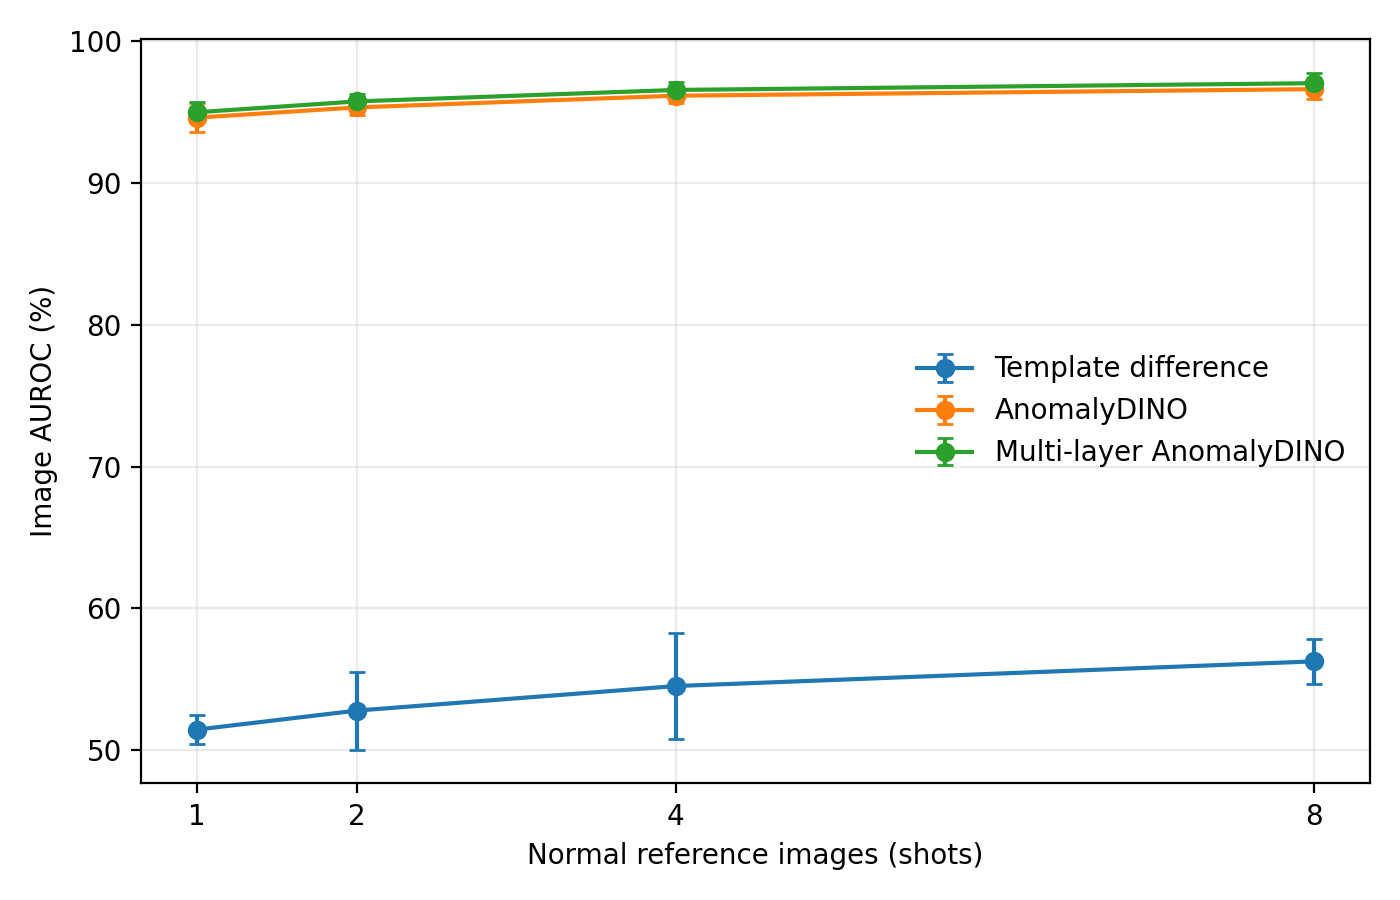
\includegraphics[width=\linewidth]{figures/image_auroc_vs_shots.png}\\
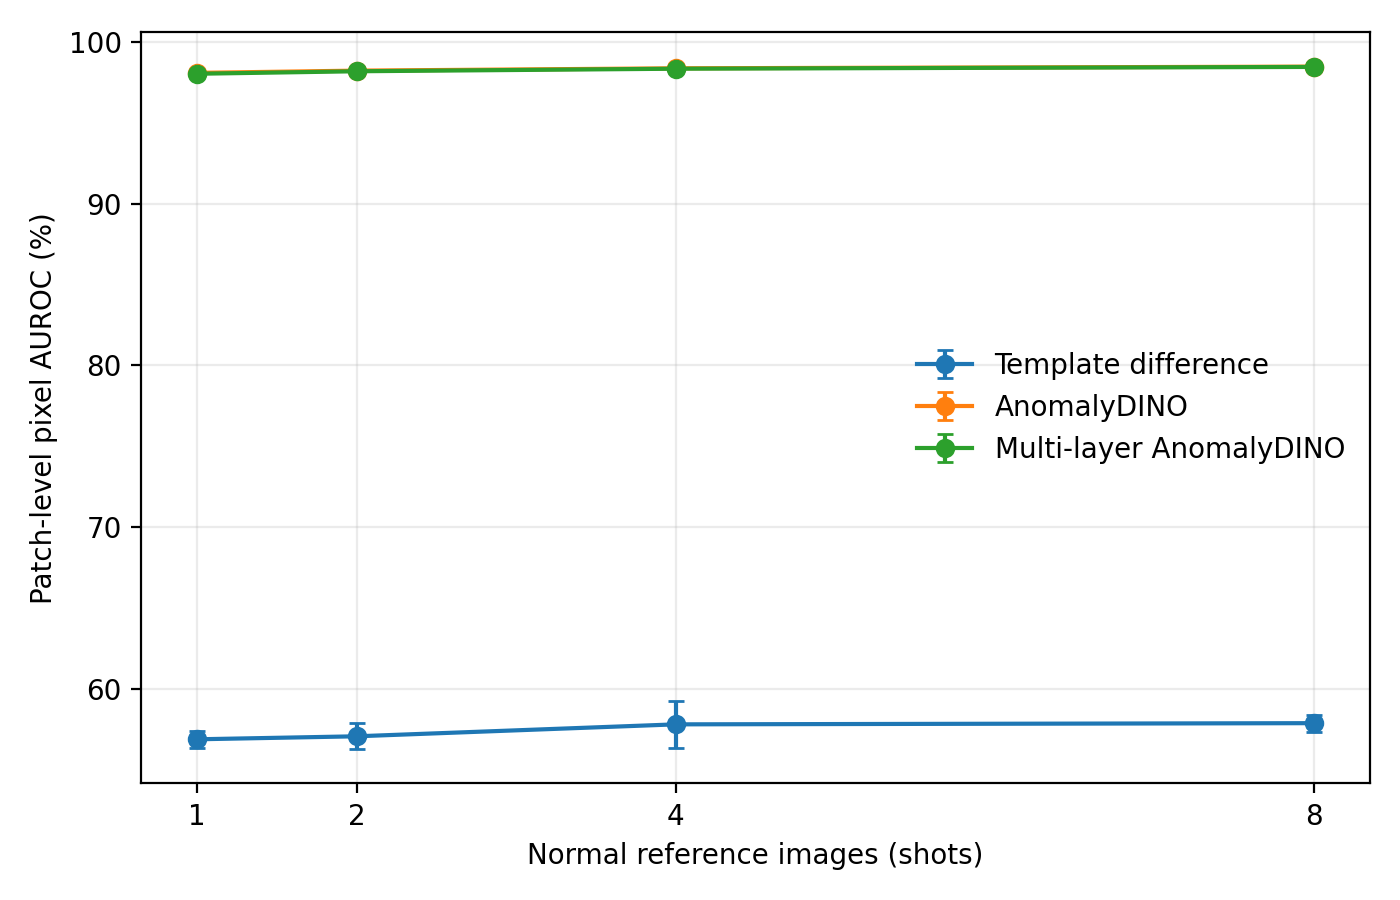
\includegraphics[width=\linewidth]{figures/pixel_auroc_vs_shots.png}
\caption{Image-level AUROC and 448-pixel localization AUROC across shot counts.
Error bars show one standard deviation over three seeds.}
\label{fig:curves}
\end{figure}

\subsection{Effect of Multi-Layer Fusion}
The improvement is intentionally conservative. It changes only how patch
features are formed, allowing changes in AUROC, AP, and localization to be
attributed to the use of blocks 9 and 11. The fused method improves image
AUROC by roughly 0.4 points at every shot count. That gain is smaller than the
seed standard deviation of 0.5--0.7 points; its direction is consistent across
all four shot settings, but we report it as a low-variance change rather than a
significant improvement. On the common 448-pixel localization grid, pixel AUROC
decreases slightly, by 0.02-0.06 points. The result is therefore presented as a
small detection/localization trade-off rather than a claim that the improvement
dominates every metric.

\subsection{Per-Category Behavior}
Large object categories such as candle provide many possible normal poses and
backgrounds, while small-object categories often have less appearance
variation but finer defects. The category table exposes this heterogeneity and
prevents one easy category from dominating the aggregate result. A high
standard deviation indicates that the chosen few references are not
interchangeable, which is a central practical risk in few-shot inspection.

\subsection{Qualitative Localization}
\begin{figure}[t]
\centering
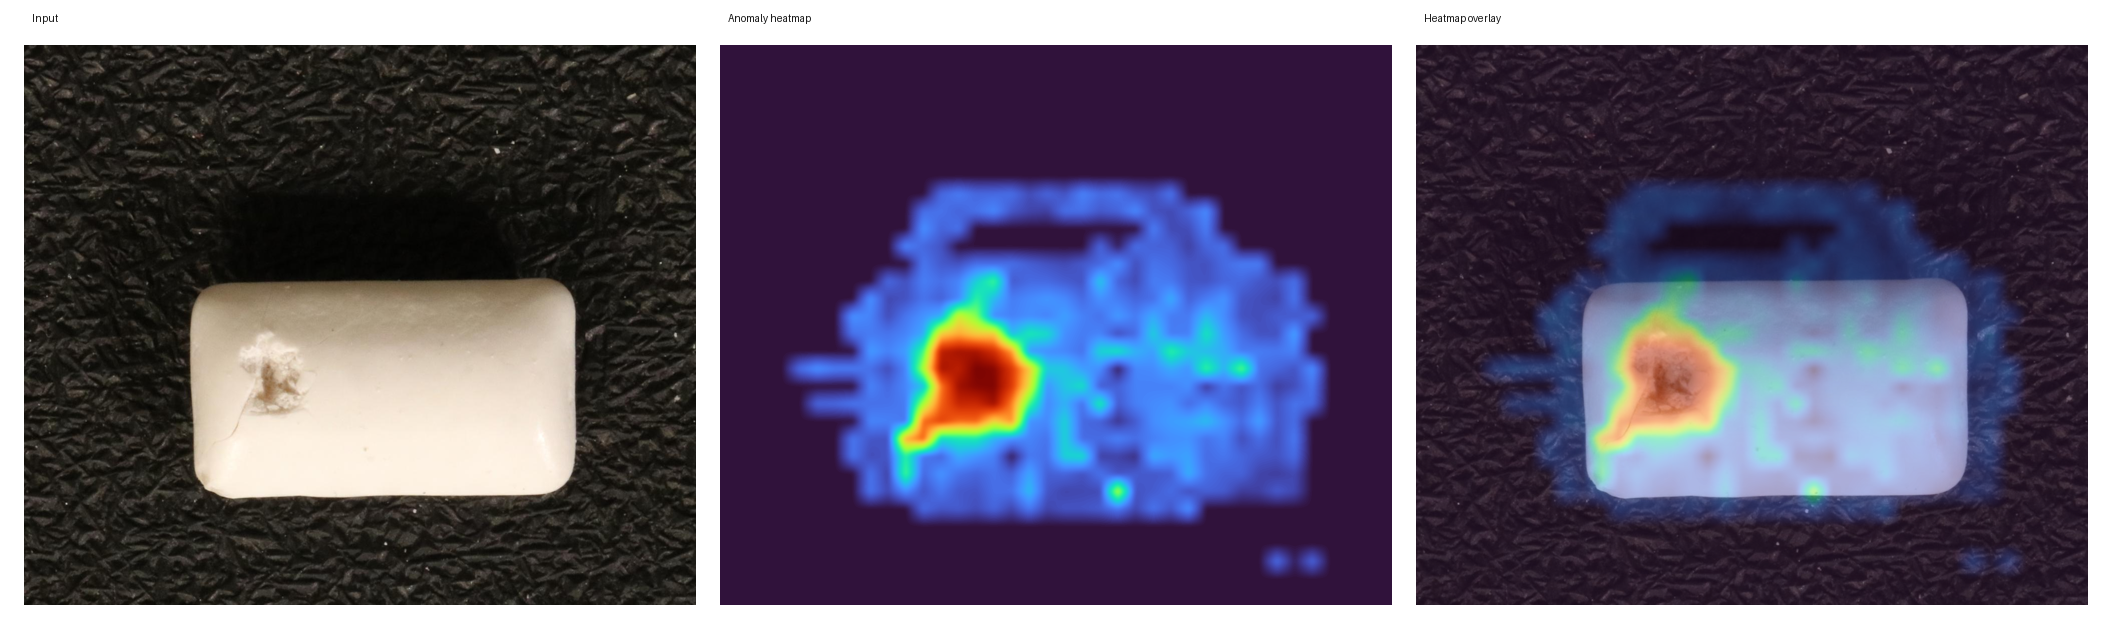
\includegraphics[width=\linewidth]{figures/qualitative_example.png}
\caption{A representative input, ground-truth mask, patch anomaly map, and
overlay. The heatmap is produced directly from AnomalyDINO distances.}
\label{fig:qualitative}
\end{figure}

Figure~\ref{fig:qualitative} shows how patch retrieval localizes an anomalous
region without any anomaly training labels. The map is intentionally coarse:
one cell covers a $14\times14$ region before upsampling. This is sufficient
for many missing-component and contamination defects but limits sub-pixel or
wire-thin defects.

\subsection{Difficult Cases}
\begin{figure*}[t]
\centering
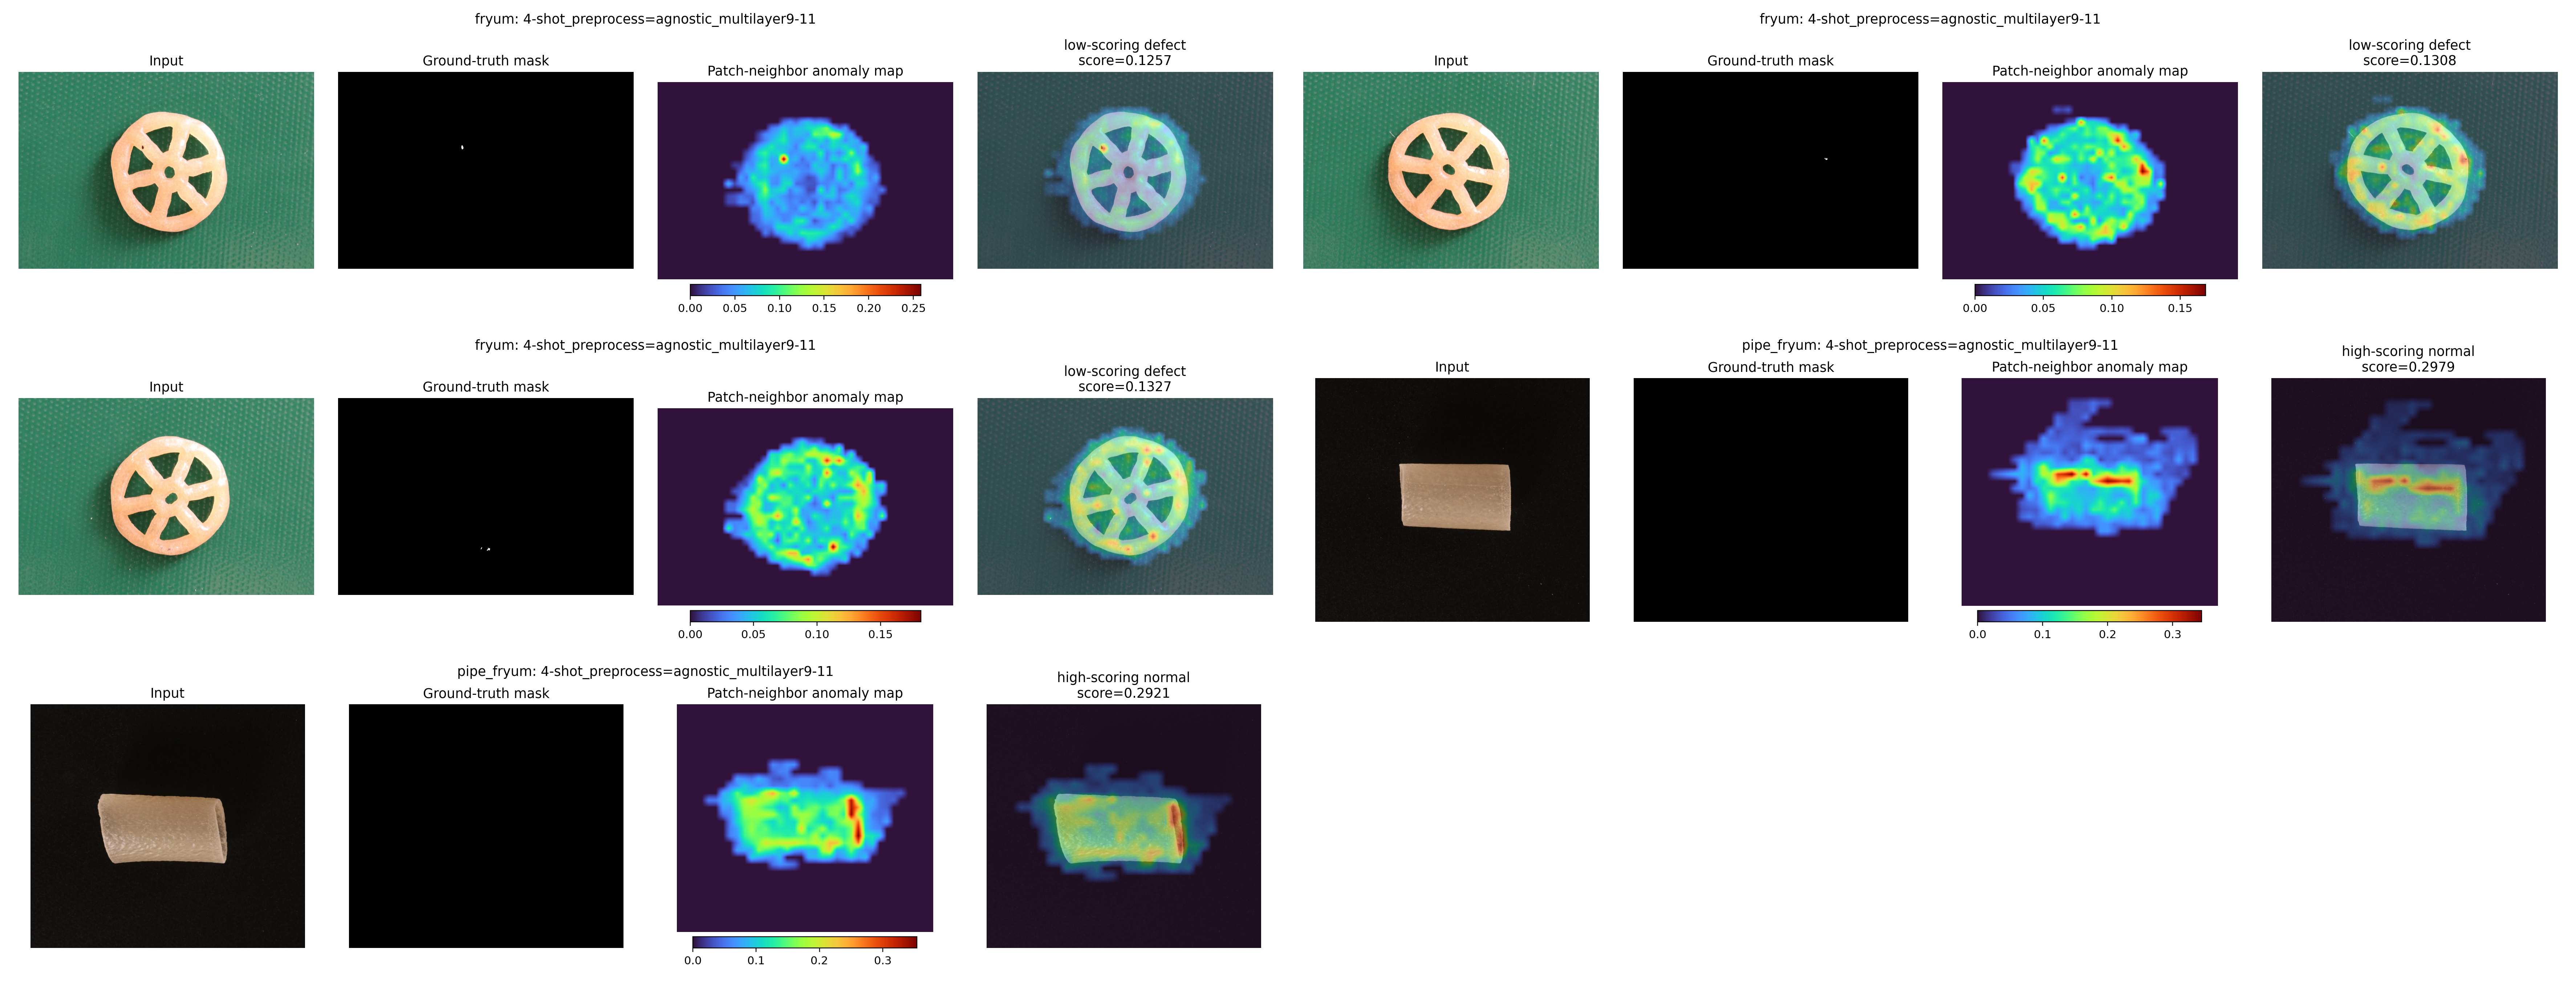
\includegraphics[width=0.96\textwidth]{figures/failure_grid.png}
\caption{Representative difficult examples selected from the actual test
errors: low-scoring defects and high-scoring normal images. Rows are not
constructed manually; cases are ranked by their unthresholded anomaly scores.}
\label{fig:failures}
\end{figure*}

Figure~\ref{fig:failures} separates two error mechanisms. Low-scoring defects
are often small or visually similar to legitimate texture variation.
High-scoring normal images usually contain a pose, reflection, or boundary
change that is represented by too few reference views. This motivates future
work on calibrated selective prediction and object-specific foreground masks.

\subsection{Efficiency}
\begin{table}[t]
\centering
\small
\caption{Encoder efficiency at $448\times448$ on an RTX A6000.}
\label{tab:efficiency}
\begin{tabular}{lrr}
\toprule
Variant & ms/image & peak GPU (MiB) \\
\midrule
AnomalyDINO & 12.2 & 132 \\
Multi-layer & 13.3 & 132 \\
\bottomrule
\end{tabular}
\end{table}


The improvement retains the same backbone and memory size, so its parameter
count and peak memory are nearly identical to the official method. The
additional cost is confined to extracting one earlier transformer block; the
nearest-neighbor database dimension remains 384.
